%%%%%%%%%%%%%%%%%%%%%%%%%%%%%%%%%%%%%%%%%
% Beamer Presentation
% LaTeX Template
% Version 1.0 (10/11/12)
%
% This template has been downloaded from:
% http://www.LaTeXTemplates.com
%
% License:
% CC BY-NC-SA 3.0 (http://creativecommons.org/licenses/by-nc-sa/3.0/)
%
%%%%%%%%%%%%%%%%%%%%%%%%%%%%%%%%%%%%%%%%%

%----------------------------------------------------------------------------------------
%	PACKAGES AND THEMES
%----------------------------------------------------------------------------------------

\documentclass{beamer}

\mode<presentation> {

% The Beamer class comes with a number of default slide themes
% which change the colors and layouts of slides. Below this is a list
% of all the themes, uncomment each in turn to see what they look like.

%\usetheme{default}
%\usetheme{AnnArbor}
%\usetheme{Antibes}
%\usetheme{Bergen}
%\usetheme{Berkeley}
%\usetheme{Berlin}
%\usetheme{Boadilla}
%\usetheme{CambridgeUS}
%\usetheme{Copenhagen}
%\usetheme{Darmstadt}
%\usetheme{Dresden}
%\usetheme{Frankfurt}
%\usetheme{Goettingen}
%\usetheme{Hannover}punto
%\usetheme{Ilmenau}
%\usetheme{JuanLesPins}punto
%\usetheme{Luebeck}
%\usetheme{Madrid}punto
%\usetheme{Malmoe}
%\usetheme{Marburg}
%\usetheme{Montpellier}punto
%\usetheme{PaloAlto}punto
%\usetheme{Pittsburgh}punto
%\usetheme{Rochester}punto
\usetheme{Singapore}
%\usetheme{Szeged}
%\usetheme{Warsaw}

% As well as themes, the Beamer class has a number of color themes
% for any slide theme. Uncomment each of these in turn to see how it
% changes the colors of your current slide theme.

%\usecolortheme{albatross}fondo azul
%\usecolortheme{beaver}titulos rojos
%\usecolortheme{beetle}fondo gris
%\usecolortheme{crane} resaltado amarillo
%\usecolortheme{dolphin} titulos azules
%\usecolortheme{dove} titulos negros
%\usecolortheme{fly} fondo gris, titulos blancos
%\usecolortheme{lily} ??
%\usecolortheme{orchid} ??
\usecolortheme{rose} %punto
%\usecolortheme{seagull} adornos gris
%\usecolortheme{seahorse} partes gris
%\usecolortheme{whale} partes azul
%\usecolortheme{wolverine} resalto amarillo

%\setbeamertemplate{footline} % To remove the footer line in all slides uncomment this line
\setbeamertemplate{footline}[page number] % To replace the footer line in all slides with a simple slide count uncomment this line

\setbeamertemplate{navigation symbols}{} % To remove the navigation symbols from the bottom of all slides uncomment this line
}

\usepackage{graphicx} % Allows including images
\usepackage{booktabs} % Allows the use of \toprule, \midrule and \bottomrule in tables
\usepackage{listings}
\usepackage{xcolor}
\usepackage{color}
%\usepackage[utf8]{inputenc}
%\usepackage[spanish]{babel}

\colorlet{punct}{red!60!black}
\definecolor{background}{HTML}{EEEEEE}
\definecolor{delim}{RGB}{25,134,57}
%\definecolor{delim}{RGB}{20,105,176}
\colorlet{numb}{magenta!60!black}

\lstdefinelanguage{json}{
    basicstyle=\normalfont\ttfamily,
    numbers=left,
    numberstyle=\scriptsize,
    stepnumber=1,
    numbersep=8pt,
    showstringspaces=false,
    breaklines=true,
    frame=lines,
    backgroundcolor=\color{background},
    literate=
     *{0}{{{\color{numb}0}}}{1}
      {1}{{{\color{numb}1}}}{1}
      {2}{{{\color{numb}2}}}{1}
      {3}{{{\color{numb}3}}}{1}
      {4}{{{\color{numb}4}}}{1}
      {5}{{{\color{numb}5}}}{1}
      {6}{{{\color{numb}6}}}{1}
      {7}{{{\color{numb}7}}}{1}
      {8}{{{\color{numb}8}}}{1}
      {9}{{{\color{numb}9}}}{1}
      {:}{{{\color{punct}{:}}}}{1}
      {,}{{{\color{punct}{,}}}}{1}
      {\{}{{{\color{delim}{\{}}}}{1}
      {\}}{{{\color{delim}{\}}}}}{1}
      {[}{{{\color{delim}{[}}}}{1}
      {]}{{{\color{delim}{]}}}}{1},
}
%----------------------------------------------------------------------------------------
%	TITLE PAGE
%----------------------------------------------------------------------------------------

\title[MongoDB]{MongoDB 3.0} % The short title appears at the bottom of every slide, the full title is only on the title page

\author{Jesse Javier Cogollo Alvarez} % Your name
\institute[EAFIT] % Your institution as it will appear on the bottom of every slide, may be shorthand to save space
{
Developer by passion \\ % Your institution for the title page
\medskip
\textit{email: cogollo87@gmail.com} % Your email address
}
\date{\today} % Date, can be changed to a custom date

\begin{document}

\begin{frame}
\titlepage % Print the title page as the first slide
\end{frame}

\begin{frame}
\frametitle{Contenido} % Table of contents slide, comment this block out to remove it
\tableofcontents % Throughout your presentation, if you choose to use \section{} and \subsection{} commands, these will automatically be printed on this slide as an overview of your presentation
\end{frame}

%----------------------------------------------------------------------------------------
%----------------------------------------------------------------------------------------
%	PRESENTATION SLIDES
%----------------------------------------------------------------------------------------

%------------------------------------------------
\section{MongoDB 3.0} % Sections can be created in order to organize your presentation into discrete blocks, all sections and subsections are automatically printed in the table of contents as an overview of the talk
%------------------------------------------------
\begin{frame}
\frametitle{@MongoDB 3.0}
\begin{figure}

\includegraphics[width=0.4\linewidth]{mongodb.png}
\end{figure}
\end{frame}
%------------------------------------------------
\begin{frame}
\frametitle{Que es @MongoDB}
'MongoDB (from "humongous") is an open-source document database, and the leading NoSQL database. Written in C++.'
{\color{blue}\url{https://www.mongodb.org/}}
\\~\\
'MongoDB was not designed in a lab. We built MongoDB from our own experiences building large-scale,high availability, robust systems...'
\underline{\color{green}Eliot Horowitz, CTO and Co-Founder}	
\end{frame}

%------------------------------------------------

\begin{frame}
\frametitle{NOSQL}
“En inform\'atica, NoSQL (a veces llamado 'no só\'olo SQL') es una amplia clase de sistemas de gesti\'on de bases de datos que difieren del modelo cl\'asico del sistema de gesti\'on de bases de datos relacionales (RDBMS) en aspectos importantes, el m\'as destacado que no usan SQL como el principal lenguaje de consultas.” {\color{blue}\url{http://es.wikipedia.org/wiki/NoSQL/}}
\\~\\

\end{frame}

%------------------------------------------------

\begin{frame}
\frametitle{Persistencia poliglota}
\begin{figure}
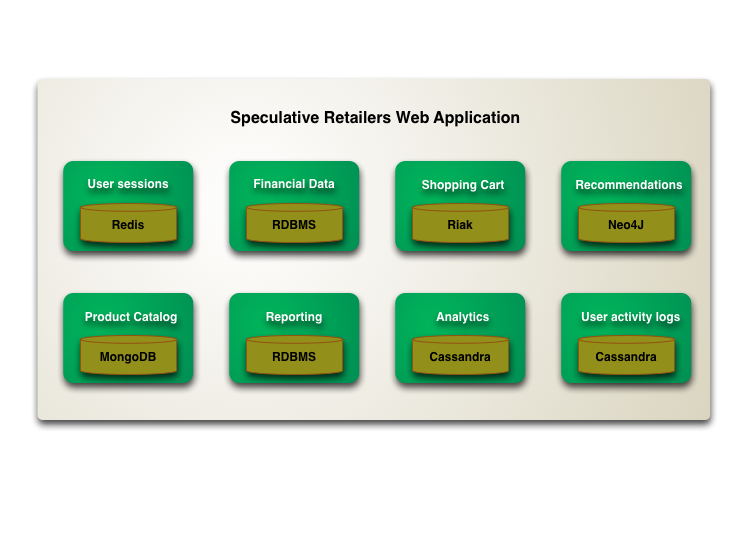
\includegraphics[width=1.0\linewidth]{polyglot.png}
\end{figure}
\end{frame}

%------------------------------------------------
\begin{frame}
\frametitle{Caracteristicas}
\begin{columns}[c] % The "c" option specifies centered vertical alignment while the "t" option is used for top vertical alignment

\column{.45\textwidth} % Left column and width
\begin{enumerate}
\item \textbf{Document-Oriented Storage}
\item[•]	
\item[•]	
\item[•]	
\item[•]	
\item[•]	
\item[•]	
\item[•]	
\end{enumerate}

\column{.5\textwidth} % Right column and width
Las \textbf{colecciones} Son esquemas dinamicos, flexibles que ofrecen simplicidad y potencia.
\begin{figure}
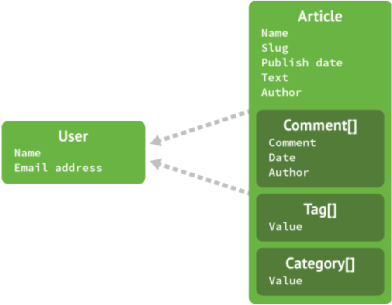
\includegraphics[width=0.9\linewidth]{document.png}
\end{figure}
\end{columns}
\end{frame}


%------------------------------------------------
\begin{frame}
\frametitle{Caracteristicas}
\begin{columns}[c] % The "c" option specifies centered vertical alignment while the "t" option is used for top vertical alignment

\column{.45\textwidth} % Left column and width
\begin{enumerate}
\item Document-Oriented Storage
\item \textbf{Full Index Support}
\item[•]	
\item[•]	
\item[•]	
\item[•]	
\item[•]	
\item[•]	
\end{enumerate}

\column{.5\textwidth} % Right column and width
Index provee alto desempeno en operaciones de lecturas.
\begin{figure}
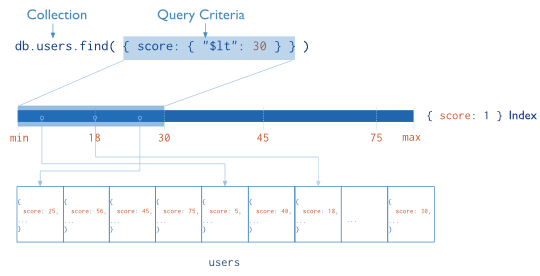
\includegraphics[width=1\linewidth]{index-with-query.png}
\end{figure}
MongoDB indexa utilizando estructura de datos B-tree.
\end{columns}
\end{frame}


%------------------------------------------------
\begin{frame}
\frametitle{Caracteristicas}
\begin{columns}[c] % The "c" option specifies centered vertical alignment while the "t" option is used for top vertical alignment

\column{.45\textwidth} % Left column and width
\begin{enumerate}
\item Document-Oriented Storage
\item Full Index Support
\item \textbf{Replication}
\item[•]	
\item[•]	
\item[•]	
\item[•]	
\item[•]	
\end{enumerate}

\column{.5\textwidth} % Right column and width
replica set en MongoDB es un grupo de procesos mongod que mantienen el mismo conjunto de datos. provee redundancia y alta disponibilidad.
\begin{figure}
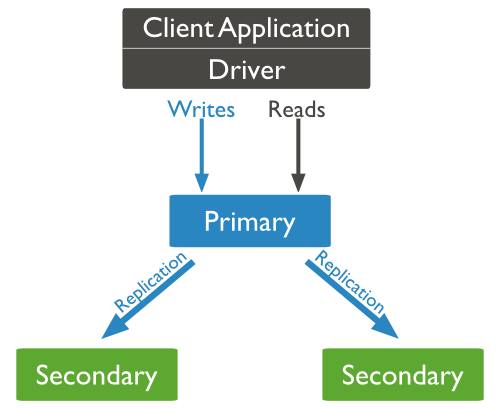
\includegraphics[width=0.6\linewidth]{replica-set-read-write-operations-primary.png}
\end{figure}
\end{columns}
\end{frame}


%------------------------------------------------
\begin{frame}
\frametitle{Caracteristicas}
\begin{columns}[c] % The "c" option specifies centered vertical alignment while the "t" option is used for top vertical alignment

\column{.45\textwidth} % Left column and width
\begin{enumerate}
\item Document-Oriented Storage
\item Full Index Support
\item Replication
\item \textbf{Auto Sharding}
\item[•]	
\item[•]	
\item[•]	
\item[•]	
\end{enumerate}

\column{.5\textwidth} % Right column and width
Escalar horizontalmente sin comprometer la funcionalidad.
\begin{figure}
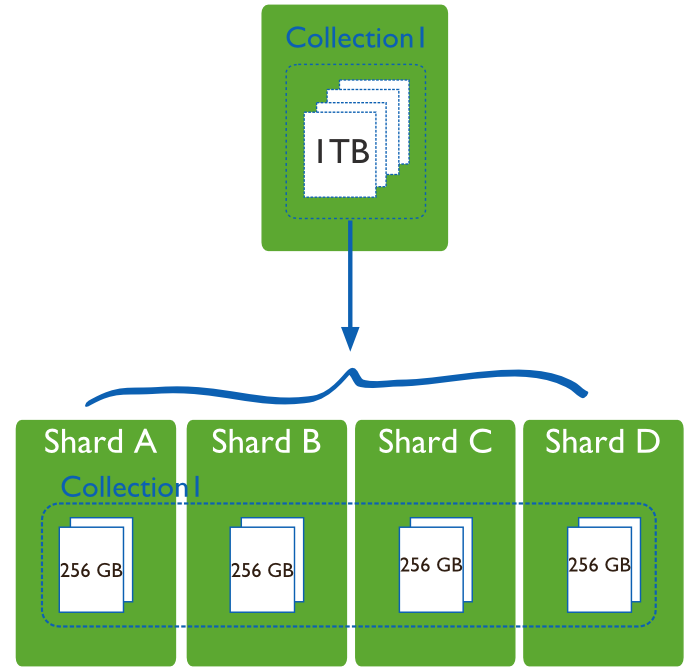
\includegraphics[width=0.8\linewidth]{sharded-collection.png}
\end{figure}
\end{columns}
\end{frame}


%------------------------------------------------
\begin{frame}
\frametitle{Caracteristicas}
\begin{columns}[c] % The "c" option specifies centered vertical alignment while the "t" option is used for top vertical alignment

\column{.45\textwidth} % Left column and width
\begin{enumerate}
\item Document-Oriented Storage
\item Full Index Support
\item Replication
\item Auto Sharding
\item \textbf{Querying}
\item[•]	
\item[•]	
\item[•]	
\end{enumerate}

\column{.5\textwidth} % Right column and width
Gran cantidad de consultas basadas en los documentos.
\begin{example}[querys]
db.collection.find(\{\})
\\~\\
db.collection.find(\{'field':'jesse'\})
\\~\\
db.inventory.find().sort(\{field:1\})
\end{example}
\end{columns}	
\end{frame}

%------------------------------------------------
\begin{frame}
\frametitle{Caracteristicas}
\begin{columns}[c] % The "c" option specifies centered vertical alignment while the "t" option is used for top vertical alignment

\column{.45\textwidth} % Left column and width
\begin{enumerate}
\item Document-Oriented Storage
\item Full Index Support
\item Replication
\item Auto Sharding
\item Querying
\item \textbf{Map Reduce}
\item[•]	
\item[•]	
\end{enumerate}

\column{.5\textwidth} % Right column and width
Map Reduce es un paradigma de procesamiento de datos para condensar grandes volumenes de datos.
\begin{figure}
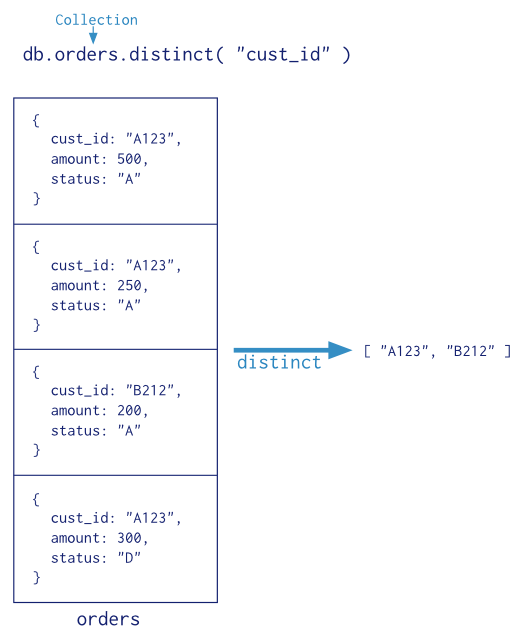
\includegraphics[width=0.5\linewidth]{distinct.png}
\end{figure}
\end{columns}
\end{frame}


%------------------------------------------------
\begin{frame}
\frametitle{Caracteristicas}
\begin{columns}[c] % The "c" option specifies centered vertical alignment while the "t" option is used for top vertical alignment

\column{.45\textwidth} % Left column and width
\begin{enumerate}
\item Document-Oriented Storage
\item Full Index Support
\item Replication
\item Auto Sharding
\item Querying
\item Map Reduce
\item \textbf{GridFS}
\item[•]	
\end{enumerate}

\column{.5\textwidth} % Right column and width
GridFS es una especificaci\'on para almacenar y recuperar archivos que exceden el limite del tamano de 16MB en los documentos BSON.
\\~\\
util utillizarlo para almacenar imagenes, audio, video, archivos de texto, etc...
\end{columns}
\end{frame}

%------------------------------------------------
\begin{frame}
\frametitle{Nuevas caracteristicas}
\begin{figure}
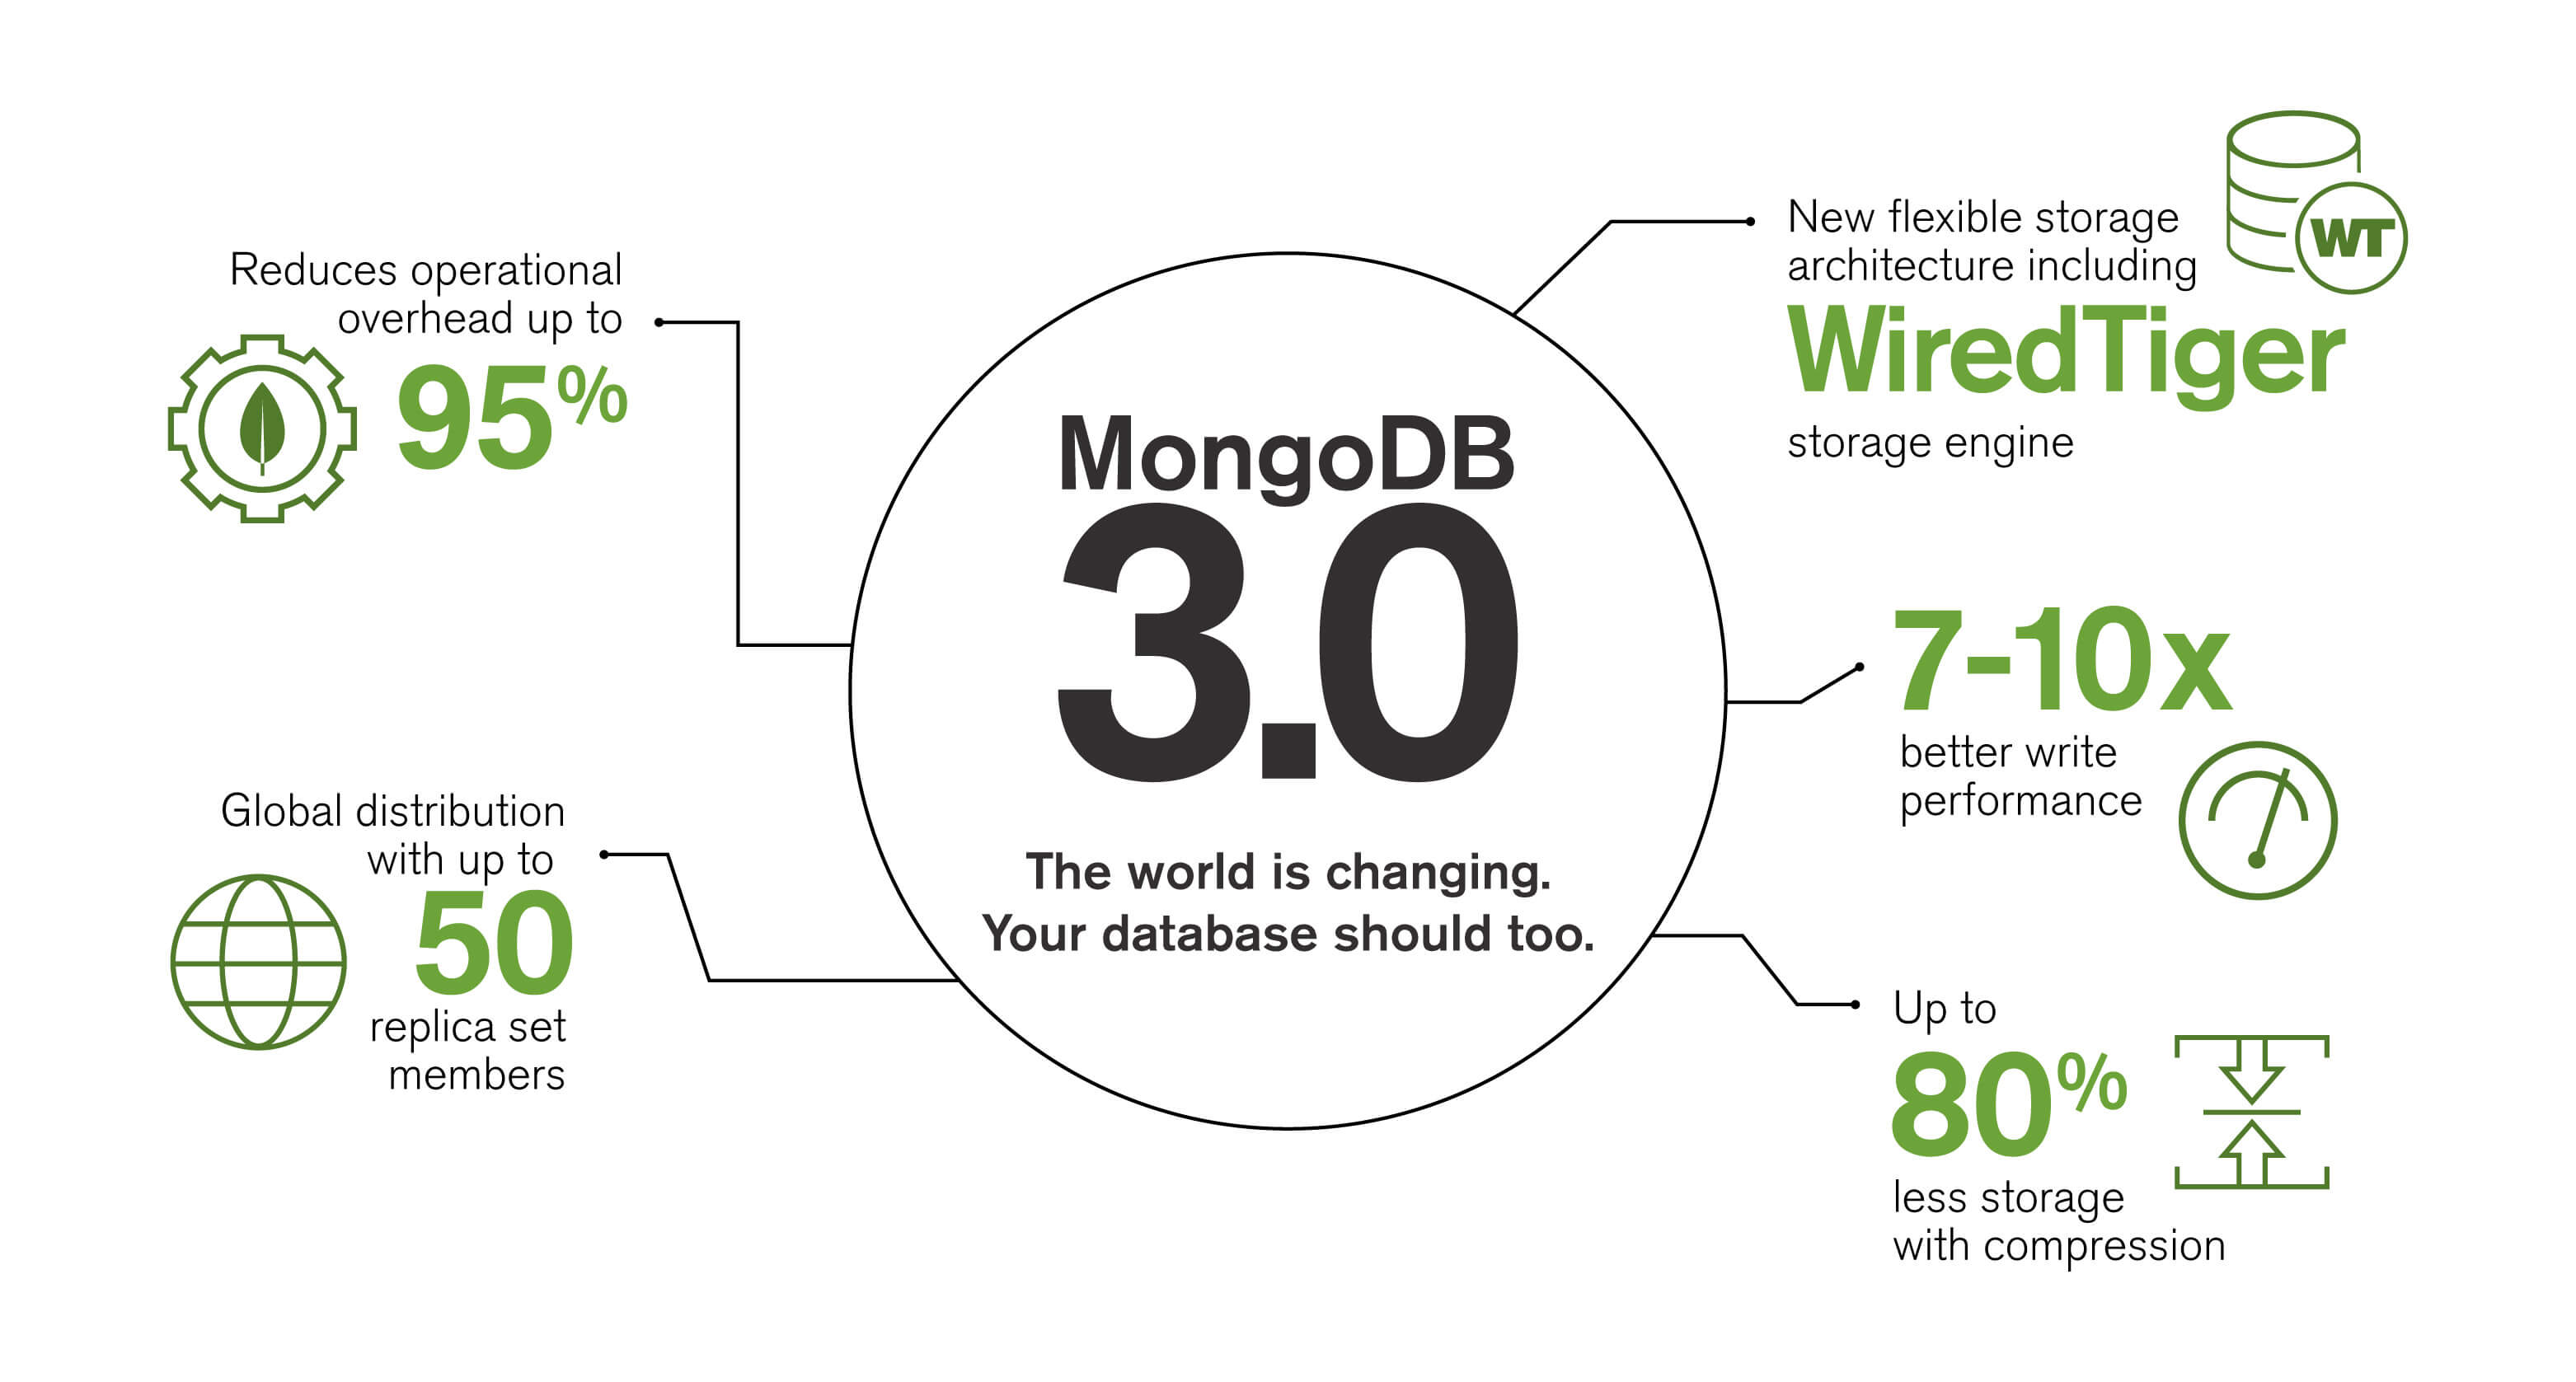
\includegraphics[width=0.8\linewidth]{mongodb3.png}
\end{figure}
\end{frame}

%------------------------------------------------
\begin{frame}
\frametitle{Nuevas caracteristicas}
\begin{columns}[c] % The "c" option specifies centered vertical alignment while the "t" option is used for top vertical alignment

\column{.45\textwidth} % Left column and width
\begin{enumerate}
\item \textbf{MongoDB Cloud}
\item[•]	
\item[•]	
\item[•]	
\item[•]	
\end{enumerate}

\column{.5\textwidth} % Right column and width
\begin{itemize}
\item MongoDB Cloud.
\end{itemize}

\end{columns}
\end{frame}

%------------------------------------------------
\begin{frame}
\frametitle{Nuevas caracteristicas}
\begin{columns}[c] % The "c" option specifies centered vertical alignment while the "t" option is used for top vertical alignment

\column{.45\textwidth} % Left column and width
\begin{enumerate}
\item MongoDB Cloud
\item \textbf{WiredTiger}
\item[•]	
\item[•]	
\item[•]	
\end{enumerate}

\column{.5\textwidth} % Right column and width
\begin{itemize}
\item
\end{itemize}

\end{columns}
\end{frame}

%------------------------------------------------
\begin{frame}
\frametitle{Nuevas caracteristicas}
\begin{columns}[c] % The "c" option specifies centered vertical alignment while the "t" option is used for top vertical alignment

\column{.45\textwidth} % Left column and width
\begin{enumerate}
\item MongoDB Cloud
\item WiredTiger
\\~\\
\textbf{Native compression}
\item[•]	
\item[•]	
\end{enumerate}

\column{.5\textwidth} % Right column and width
Options:
\begin{itemize}
\item No compression
\item Snappy (default)
\item zlib (similar to gzip)
\end{itemize}

Options indexes:
\begin{itemize}
\item No compression
\item Prefix (default)
\end{itemize}

\end{columns}
\end{frame}

%------------------------------------------------
\begin{frame}
\frametitle{Nuevas caracteristicas}
\begin{columns}[c] % The "c" option specifies centered vertical alignment while the "t" option is used for top vertical alignment

\column{.45\textwidth} % Left column and width
\begin{enumerate}
\item MongoDB Cloud
\item WiredTiger
\\~\\
\textbf{Puggable}
\item[•]	
\item[•]	
\end{enumerate}

\column{.5\textwidth} % Right column and width
\begin{figure}
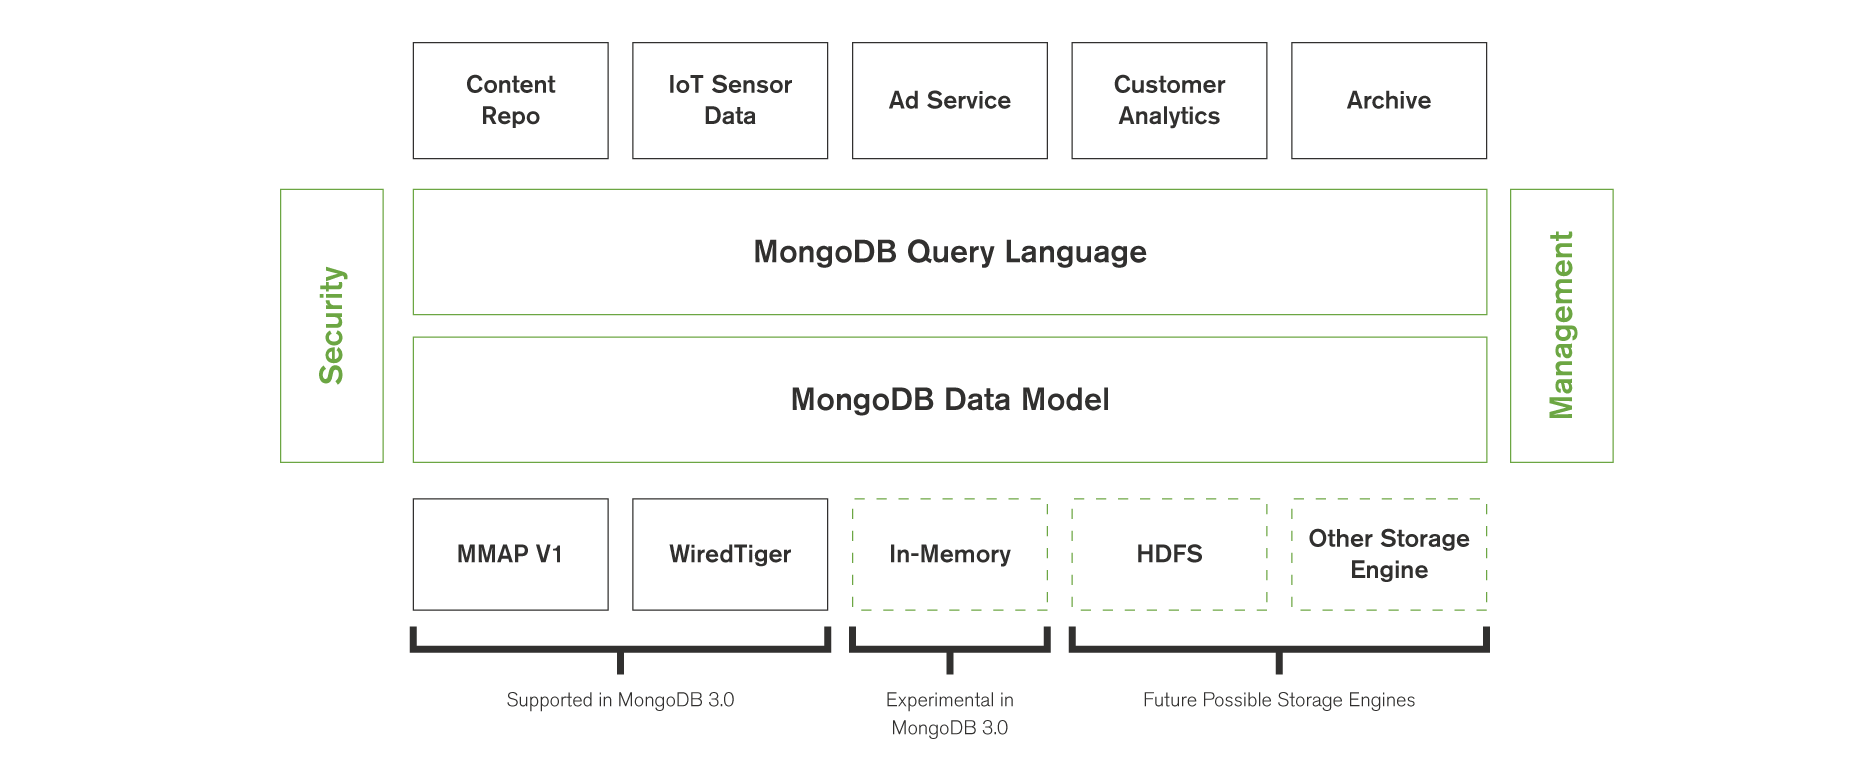
\includegraphics[width=1\linewidth]{pluggable.png}
\end{figure}
\end{columns}
\end{frame}

%------------------------------------------------
\begin{frame}
\frametitle{Nuevas caracteristicas}
\begin{columns}[c] % The "c" option specifies centered vertical alignment while the "t" option is used for top vertical alignment

\column{.45\textwidth} % Left column and width
\begin{enumerate}
\item MongoDB Cloud
\item WiredTiger
\item \textbf{queries}
\item[•]	
\item[•]	
\end{enumerate}

\column{.5\textwidth} % Right column and width
\begin{itemize}
\item explain()
\item Multi-Hemisphere Queries
\item \$dateToString
\end{itemize}
\end{columns}
\end{frame}

%------------------------------------------------
\begin{frame}[fragile] % Need to use the fragile option when verbatim is used in the slide
\frametitle{quiero empezar con WiredTiger}
\textbf{Desde Terminal}
\begin{lstlisting}[language=json,firstnumber=1]
mongod --storageEngine wiredTiger
\end{lstlisting}
\end{frame}

%------------------------------------------------

\begin{frame}
\frametitle{Administradores graficos}
\begin{columns}[c] % The "c" option specifies centered vertical alignment while the "t" option is used for top vertical alignment

\column{.45\textwidth} % Left column and width
\textbf{•}
\begin{enumerate}
\item \textbf{Robomongo}
\item[•]
\item[•]
\end{enumerate}

\column{.5\textwidth} % Right column and width
{\color{blue}\url{http://goo.gl/rLEUYg}}
\end{columns}

\end{frame}

%------------------------------------------------
\begin{frame}
\frametitle{Administradores graficos}
\begin{columns}[c] % The "c" option specifies centered vertical alignment while the "t" option is used for top vertical alignment

\column{.45\textwidth} % Left column and width
\textbf{•}
\begin{enumerate}
\item Robomongo
\item \textbf{Ridemongo}
\item[•]
\end{enumerate}

\column{.5\textwidth} % Right column and width
{\color{blue}\url{http://goo.gl/XmH7bj}}
\end{columns}
\end{frame}

%------------------------------------------------
\begin{frame}
\frametitle{Administradores graficos}
\begin{columns}[c] % The "c" option specifies centered vertical alignment while the "t" option is used for top vertical alignment

\column{.45\textwidth} % Left column and width
\textbf{•}
\begin{enumerate}
\item Robomongo
\item Ridemongo
\item \textbf{Muchos mas...}
\end{enumerate}

\column{.5\textwidth} % Right column and width
{\color{blue}\url{http://goo.gl/uaJJiZ}}
\end{columns}

\end{frame}

%------------------------------------------------
\begin{frame}
\frametitle{Insert Find Update Remove (CRUD)}
\begin{block}{\textbf{I}FUR}
db.collection.insert(\{"name":"jesse","age":28\})
\end{block}
\begin{block}{I\textbf{F}UR}
db.collection.find(\{"name":"jesse"\})
\end{block}
\begin{block}{IF\textbf{U}R}
db.collection.update(\{"name":"jesse"\},
\{\$set:\{"age":20\}\})
\end{block}
\begin{block}{IFU\textbf{R}}
db.collection.remove(\{"name":"jesse"\})
\end{block}
\end{frame}

%------------------------------------------------
\section{MongoDB Medellin}
%------------------------------------------------
\begin{frame}
\frametitle{MongoDB Medellin}
\begin{figure}

\includegraphics[width=0.3\linewidth]{mongodbmedellin.png}
\end{figure}
\end{frame}
%------------------------------------------------
\begin{frame}
\frametitle{Redes sociales}
\begin{columns}[c] % The "c" option specifies centered vertical alignment while the "t" option is used for top vertical alignment

\column{.45\textwidth} % Left column and width
\begin{enumerate}
\item \textbf{Meetup}
\item[•]	
\item[•]	
\item[•]	
\item[•]	
\item[•]	
\end{enumerate}

\column{.5\textwidth} % Right column and width
{\color{blue}/MongoDB-Medellin}
\\~\\
{\color{blue}\url{http://goo.gl/fw5Gyh}}
\end{columns}
\end{frame}
%------------------------------------------------

\begin{frame}
\frametitle{Redes sociales}
\begin{columns}[c] % The "c" option specifies centered vertical alignment while the "t" option is used for top vertical alignment

\column{.45\textwidth} % Left column and width
\begin{enumerate}
\item Meetup
\item \textbf{Twitter}
\item[•]	
\item[•]	
\item[•]	
\item[•]	
\end{enumerate}

\column{.5\textwidth} % Right column and width
{\color{blue}@mongodbmedelln}
\\~\\
{\color{blue}\url{http://goo.gl/gdCAjF}}
\end{columns}
\end{frame}
%------------------------------------------------

\begin{frame}
\frametitle{Redes sociales}
\begin{columns}[c] % The "c" option specifies centered vertical alignment while the "t" option is used for top vertical alignment

\column{.45\textwidth} % Left column and width
\begin{enumerate}
\item Meetup
\item Twitter
\item \textbf{Facebook}
\item[•]	
\item[•]	
\item[•]	
\end{enumerate}

\column{.5\textwidth} % Right column and width
{\color{blue}/MongoDBMedellin}
\\~\\
{\color{blue}\url{http://goo.gl/Q1JnXQ}}
\end{columns}
\end{frame}
%------------------------------------------------	
\begin{frame}
\frametitle{Redes sociales}
\begin{columns}[c] % The "c" option specifies centered vertical alignment while the "t" option is used for top vertical alignment

\column{.45\textwidth} % Left column and width
\begin{enumerate}
\item Meetup
\item Twitter
\item Facebook
\item \textbf{Google Plus}
\item[•]	
\item[•]	
\end{enumerate}

\column{.5\textwidth} % Right column and width
{\color{blue}+ MongoDBMedellin}
\\~\\
{\color{blue}\url{http://goo.gl/5VtG1h}}
\end{columns}
\end{frame}
%------------------------------------------------	
\begin{frame}
\frametitle{Redes sociales}
\begin{columns}[c] % The "c" option specifies centered vertical alignment while the "t" option is used for top vertical alignment

\column{.45\textwidth} % Left column and width
\begin{enumerate}
\item Meetup
\item Twitter
\item Facebook
\item Google Plus
\item \textbf{Lista de correo}
\item[•]	
\end{enumerate}

\column{.5\textwidth} % Right column and width
{\color{blue}+ correo}
\\~\\
{\color{blue}\url{http://goo.gl/FJvrjT}}
\end{columns}
\end{frame}
%------------------------------------------------	
\begin{frame}
\frametitle{Redes sociales}
\begin{columns}[c] % The "c" option specifies centered vertical alignment while the "t" option is used for top vertical alignment

\column{.45\textwidth} % Left column and width
\begin{enumerate}
\item Meetup
\item Twitter
\item Facebook
\item Google Plus
\item Lista de correo
\item \textbf{Grupo de estudio}
\end{enumerate}

\column{.5\textwidth} % Right column and width
%\begin{figure}
%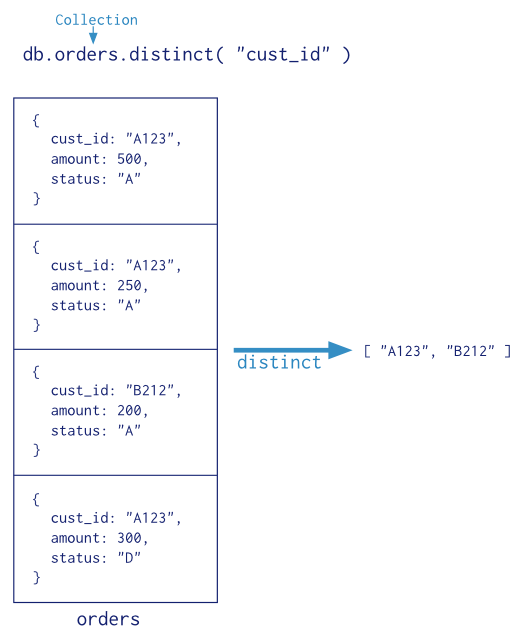
\includegraphics[width=0.5\linewidth]{distinct.png}
%\end{figure}
{\color{blue}Formulario grupo de estudio}
\\~\\
{\color{blue}\url{http://goo.gl/7ALdst}}
\end{columns}
\end{frame}
%------------------------------------------------	
\begin{frame}
\frametitle{Donde aprender}
\begin{columns}[c] % The "c" option specifies centered vertical alignment while the "t" option is used for top vertical alignment
\column{.45\textwidth} % Left column and width
\begin{enumerate}
\item \textbf{Download}
\item[•]
\item[•]
\item[•]
\item[•]
\item[•]
\item[•]
\end{enumerate}

\column{.5\textwidth} % Right column and width
%\begin{figure}
%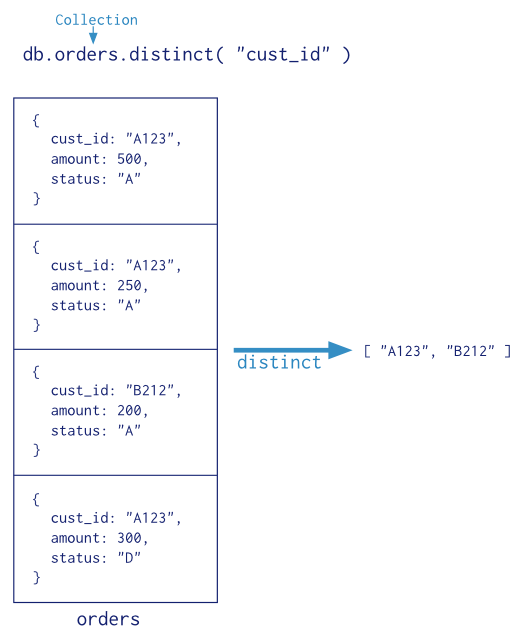
\includegraphics[width=0.5\linewidth]{distinct.png}
%\end{figure}
{\color{blue}\url{https://www.mongodb.org/downloads}}
\end{columns}
\end{frame}
%------------------------------------------------	
\begin{frame}
\frametitle{Donde aprender}
\begin{columns}[c] % The "c" option specifies centered vertical alignment while the "t" option is used for top vertical alignment
\column{.45\textwidth} % Left column and width
\begin{enumerate}
\item Download
\item \textbf{Training}
\item[•]
\item[•]
\item[•]
\item[•]
\item[•]
\end{enumerate}

\column{.5\textwidth} % Right column and width
%\begin{figure}
%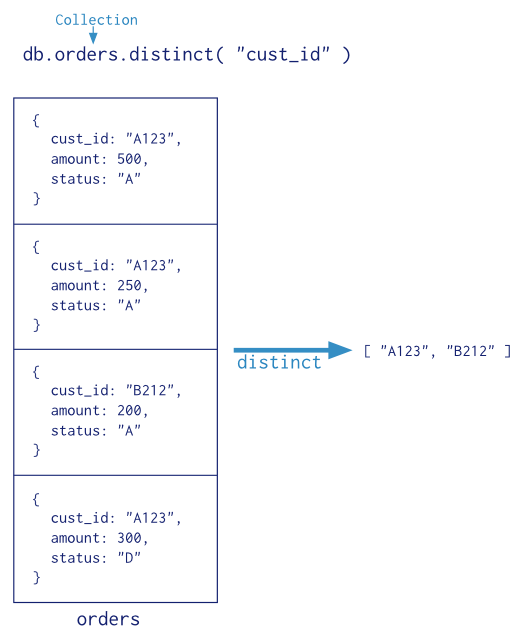
\includegraphics[width=0.5\linewidth]{distinct.png}
%\end{figure}
{\color{blue}\url{https://university.mongodb.com/courses/catalog}}
\end{columns}
\end{frame}
%------------------------------------------------	
\begin{frame}
\frametitle{Donde aprender}
\begin{columns}[c] % The "c" option specifies centered vertical alignment while the "t" option is used for top vertical alignment
\column{.45\textwidth} % Left column and width
\begin{enumerate}
\item Download
\item Training
\item \textbf{Webinar and Events}
\item[•]
\item[•]
\item[•]
\item[•]
\end{enumerate}

\column{.5\textwidth} % Right column and width
%\begin{figure}
%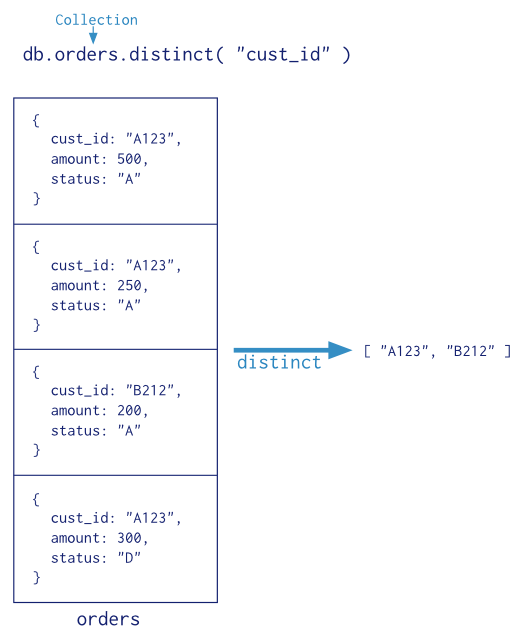
\includegraphics[width=0.5\linewidth]{distinct.png}
%\end{figure}
{\color{blue}\url{http://www.mongodb.com/webinars}}
\end{columns}
\end{frame}
%------------------------------------------------	
\begin{frame}
\frametitle{Donde aprender}
\begin{columns}[c] % The "c" option specifies centered vertical alignment while the "t" option is used for top vertical alignment
\column{.45\textwidth} % Left column and width
\begin{enumerate}
\item Download
\item Training
\item Webinar and Events
\item \textbf{White papers}
\item[•]
\item[•]
\item[•]
\end{enumerate}

\column{.5\textwidth} % Right column and width
%\begin{figure}
%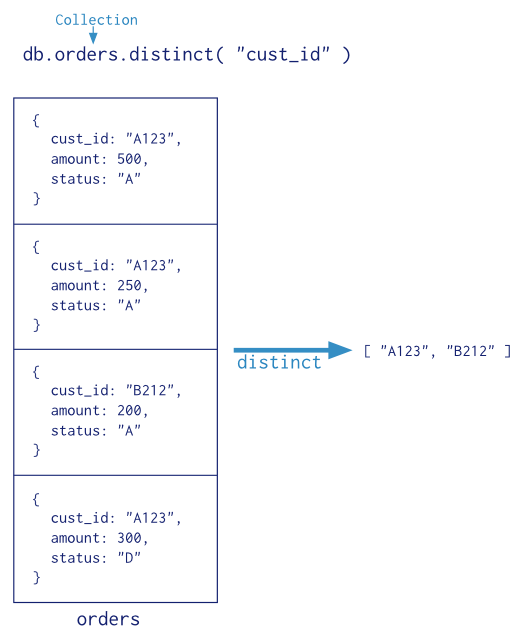
\includegraphics[width=0.5\linewidth]{distinct.png}
%\end{figure}
{\color{blue}\url{http://www.mongodb.com/white-papers}}
\end{columns}
\end{frame}
%------------------------------------------------	
\begin{frame}
\frametitle{Donde aprender}
\begin{columns}[c] % The "c" option specifies centered vertical alignment while the "t" option is used for top vertical alignment
\column{.45\textwidth} % Left column and width
\begin{enumerate}
\item Download
\item Training
\item Webinar and Events
\item White papers
\item \textbf{Case studies}
\item[•]
\item[•]
\end{enumerate}

\column{.5\textwidth} % Right column and width
%\begin{figure}
%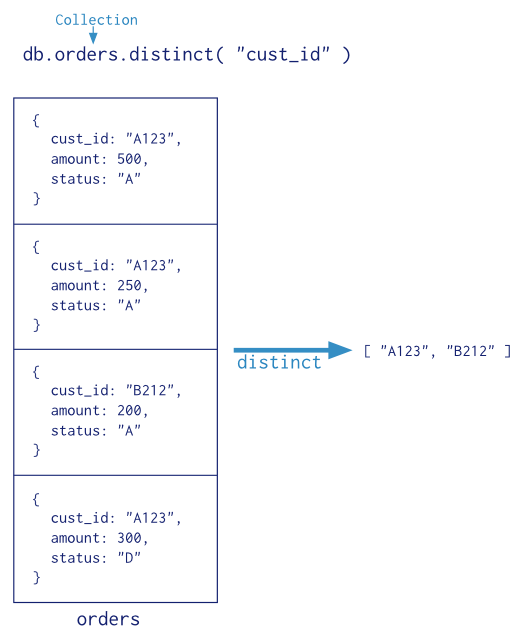
\includegraphics[width=0.5\linewidth]{distinct.png}
%\end{figure}
{\color{blue}\url{http://www.mongodb.com/who-uses-mongodb}}
\end{columns}
\end{frame}
%------------------------------------------------	
\begin{frame}
\frametitle{Donde aprender}
\begin{columns}[c] % The "c" option specifies centered vertical alignment while the "t" option is used for top vertical alignment
\column{.45\textwidth} % Left column and width
\begin{enumerate}
\item Download
\item Training
\item Webinar and Events
\item White papers
\item Case studies
\item \textbf{Presentations}
\item[•]
\end{enumerate}

\column{.5\textwidth} % Right column and width
%\begin{figure}
%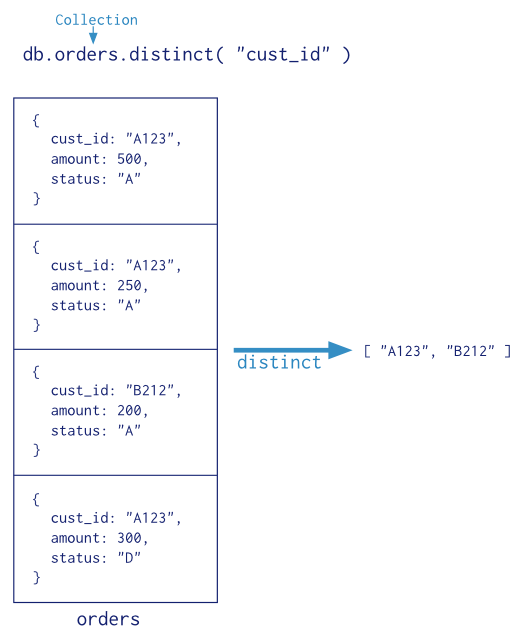
\includegraphics[width=0.5\linewidth]{distinct.png}
%\end{figure}
{\color{blue}\url{http://www.mongodb.com/presentations/all}}
\end{columns}
\end{frame}
%------------------------------------------------	
\begin{frame}
\frametitle{Donde aprender}
\begin{columns}[c] % The "c" option specifies centered vertical alignment while the "t" option is used for top vertical alignment
\column{.45\textwidth} % Left column and width
\begin{enumerate}
\item Download
\item Training
\item Webinar and Events
\item White papers
\item Case studies
\item Presentations
\item \textbf{Documentation}
\end{enumerate}

\column{.5\textwidth} % Right column and width
%\begin{figure}
%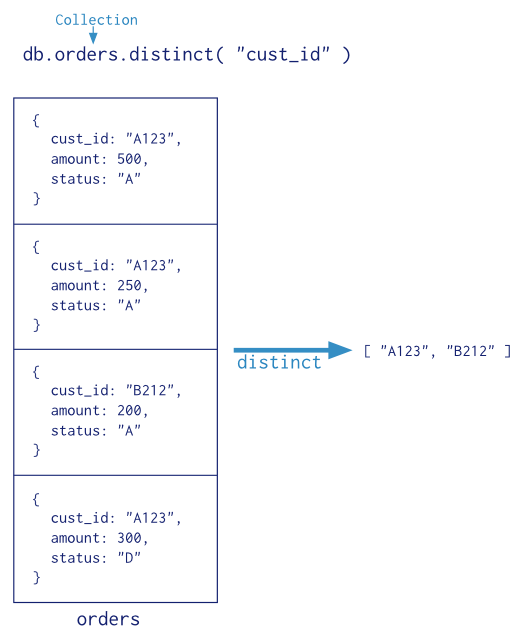
\includegraphics[width=0.5\linewidth]{distinct.png}
%\end{figure}
{\color{blue}\url{http://docs.mongodb.org/manual/}}
\end{columns}
\end{frame}
%------------------------------------------------	
\begin{frame}
\frametitle{Links de referencia}
\footnotesize{
\begin{thebibliography}{99} % Beamer does not support BibTeX so references must be inserted manually as below
\bibitem[]{p1} JSON
\newblock http://json.org/
\end{thebibliography}
}
\footnotesize{
\begin{thebibliography}{99} % Beamer does not support BibTeX so references must be inserted manually as below
\bibitem[]{p1} Documentaci\'on y Recursos
\newblock https://www.mongodb.org/
\end{thebibliography}
}
\footnotesize{
\begin{thebibliography}{99} % Beamer does not support BibTeX so references must be inserted manually as below
\bibitem[]{p1} MongoDB Cloud
\newblock https://www.mongodb.com/
\end{thebibliography}
}
\end{frame}

%------------------------------------------------
\begin{frame}
\frametitle{Demo}

\end{frame}

%------------------------------------------------
\begin{frame}
\frametitle{Preguntas}
\begin{figure}

\includegraphics[width=0.4\linewidth]{preguntas.png}
\end{figure}
\end{frame}

%------------------------------------------------
\begin{frame}
\Huge{\centerline{Gracias !!! =)}}
\end{frame}

%----------------------------------------------------------------------------------------

\end{document} 
